\documentclass{article}
\usepackage[utf8]{inputenc}
\usepackage{datetime}
\usepackage{enumerate}
\usepackage{textcomp}
\usepackage{amsmath}
\usepackage{tikz}
\usetikzlibrary{arrows}
\usepackage{graphicx}
\usepackage{amssymb}
\graphicspath{ {./images/} }
   
\title{\bf \Large ASSIGNMENT 9}
\author{Xinhao Luo}
\date{\today}

\def\math#1{$#1$} 

\setlength{\textheight}{8.5in}
\setlength{\textwidth}{6.5in}
\setlength{\oddsidemargin}{0in}
\setlength{\evensidemargin}{0in}
\voffset0.0in

\begin{document}
\maketitle
\medskip

\section{Question 1}

The 8th order polynomial feature transform will have \math{\sum_{n=1}^8 n = 45} features, and we have 300 samples. The dimension of Z will be \math{300 \times 45}

\section{Question 2}

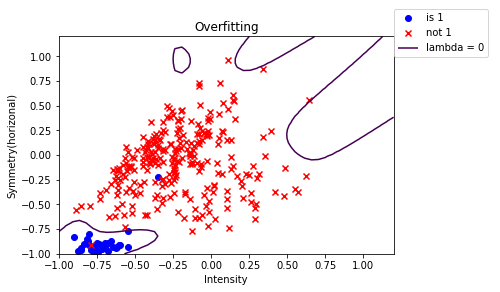
\includegraphics[]{2/1}

There is overfitting

\section{Question 3}

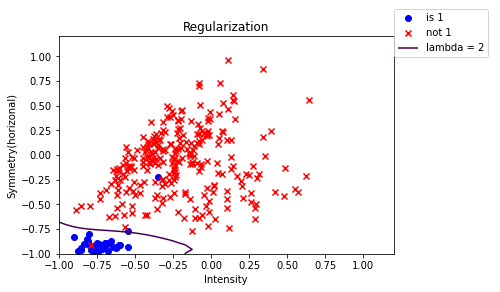
\includegraphics[]{3/1}

A little underfitting.

\section{Question 4}

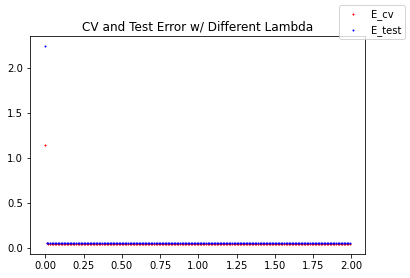
\includegraphics[]{4/1}

\math{E_{cv}} is always smaller than \math{E_{test}}. Still, they share the same trend, which means \math{E_{cv}} reflects the changes of \math{E_{test}}

\section{Question 5}

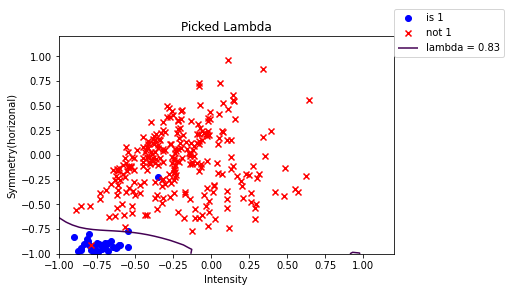
\includegraphics[]{5/1}
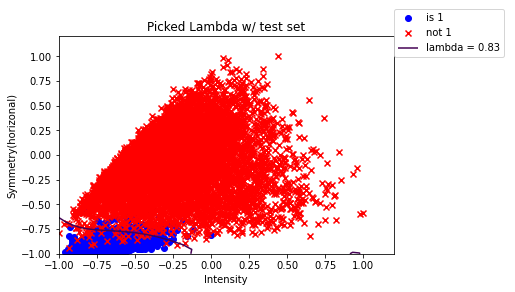
\includegraphics[]{5/2}

\section{Question 6} 

Given that \math{\lambda = 0.83}, \math{E_{test}: 0.04801203670522442}, \math{N = 8998}, \math{\delta = 0.01}

\begin{equation}
    E_{out} < E_{test} + \sqrt{\frac{1}{2N} ln\frac{2M}{\delta}} = 0.048012 + \sqrt{\frac{1}{8998 \times 2}ln\frac{2 \times 1}{0.01}} = 0.06517
\end{equation}

Thus it is saying we have \math{99\%} confidence that \math{E_{out}} is less than \math{0.06517} 

\section{Question 7}

No, it is unbiased, since each validation we have the test data out of the training process. \math{E_{cv}} is calculated from \math{g^-} (\math{N - 1}), and \math{\lambda^*} is chosen based \math{E_{cv}}.


\section{Question 8}

No, it is biased, since 1) we separate the data into training and test; 2) we compute \math{\lambda*} based on training set; 3) we calculate \math{E_{test}(w_{reg}(\lambda*))} after \math{\lambda*} has computed, which is where the data snooping happened. To fix it, we may have different set of data at the beginning so that choosing training data won't affect the selection of testing data then the problem solved.

\end{document}
